\documentclass[12pt]{article}

% packages
\usepackage{a4wide}
\usepackage[english]{babel}
\usepackage{csquotes}
\usepackage{float}
\usepackage{hyperref}
\usepackage{subcaption}
\usepackage{listings}
\usepackage{xcolor}
\usepackage{enumitem}
\usepackage{fontenc}
\usepackage{inputenc}
\usepackage{graphicx}
\usepackage{wrapfig}
\usepackage{tocloft}
\usepackage{array}

\usepackage{biblatex}
\addbibresource{../biblio.bib}

% formatting
\renewcommand{\cftsecleader}{\cftdotfill{\cftdotsep}}   % points in table of contents
\setlength{\parskip}{\baselineskip}                     % add space between paragraphs

\lstset{
    captionpos=b,
    label={lst:script},
    basicstyle=\scriptsize\ttfamily,
    keywordstyle=\color{blue},
    commentstyle=\color{green!60!black},
    numbers=left,
    numberstyle=\tiny\color{gray},
    abovecaptionskip=0.8cm
}


% attributes
\title{\underline{\textbf{ExaMA WP3 -- Dashboard Performances}}}
\author{Tanguy Pierre\\
            [1cm]
            Supervisors: V. Chabannes, J. Cladellas\\
            [2cm]
            University of Strasbourg}

\date{31st of May}


% **********************  START  **********************
\begin{document}
    \maketitle      % titlepage to be improved

\newpage
\tableofcontents


\newpage
\section{Introduction}

This work is part of the \textit{ExaMA} project, which falls under the French program \textit{NumPEx}\cite*{NumPEx}.
NumPEx is highly active across various research domains of HPC, but the ExaMa project focuses primarily on methods and algorithms and their adaptation to exascale computing. \\
Exascale \textit{exascale} machines are capable of performing $1$ exaflop, or $10^{18}$ operations per second, highlighting the need for algorithms and methods to be robust and performant.

Algorithms may experience terrible performances on, or near, exascale machines.
The complex communication between the numerous cores is often the reason for this.
In order to control the methods and their performances, they must be tested them under different conditions.

In the following graphic, you can see the organisation of the \textit{ExaMa} project.
The \textit{Dashboard performance} project is positioned between WP3 and WP7, as its objective is to develop a benchmarking platform for the solvers from WP3.
\newline
\begin{figure}[h]
    \centering
    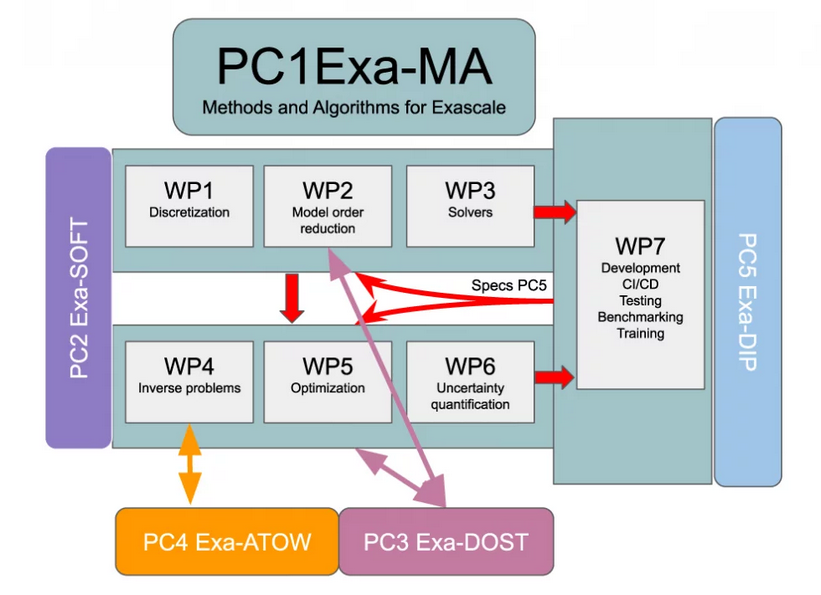
\includegraphics[width=0.6\textwidth]{../illustrations/ExaMa-orga.png}
\end{figure}

Benchmarking is an essential step for \textit{ExaMA}, as it needs to analyse and compare performances on systems
with different structures. These analyses will not only guide the developer team in improving the scalability of the different available tools,
but also ensure complete transparency about the evaluation process.

\newpage
As launching tests on supercomputers isn't always easy because of their availability and costs, there is a real need to have fast-deployable test programs and to store the results efficiently.
Additionally, this serves as a manner to verify that new features haven't caused any pullback in performance. \\
Storing the results will provide a possibility to perform analyses depending on specific context, such as machine or application.
Therefore, it is also crucial for the project to create a well-structured database in order to get a clear overview.

It is exactly what the \textit{Dashboard Performances} project aims to achieve: providing a clear and easy-to-use interface between tests and results.
This interface is already available at \url{https://feelpp.github.io/benchmarking/benchmarking/index.html}.

\vspace{1cm}
\section{Objectives}
\begin{itemize}
    \item Establish a \textbf{Continuous Integration/Continuous Deployment} workflow.
    This means that every time a new test is executed and integrated into the repository main branch, a task will automatically be launched for updating the documentation site. \\
    \item Improve the \textbf{dashboard presentation}. We need to enhance the data visualization and to provide explanations for a better comprehension of the results. \\
    \item Provide a \textbf{database} for easy access and retrieval of test results.
    Currently, it is very difficult to perform clear data analysis based on different aggregations, as it requires manual searching.
    Therefore, we want to develop an automated solution to select relevant fields.
    \item Identifiying appropriate values for performance analysis on specific context can be challenging. Therefore, conducting \textbf{representative tests} is essential to obtain reliable results about the system's behaviour. \\


\end{itemize}

\newpage
\section{Tools}

For testing the implemented algorithms and predicting how they will behave, we will use \textit{ReFrame HPC}\cite*{ReFrame}.
ReFrame is a robust framework based on Python classes that allows us to focus only on the algorithm by isolating the running code from the system's complexity.
The interesting aspect of this framework is that it allows launching multiple tests at once, ensuring their sanity, and extracting performance metrics.
Furthermore, its pipeline allows to create tests for specific stages of the program, such as the compilation or execution phase. 
For our purpose, we will only use the execution testing part of it.

The algorithms we want to test will be from the \textit{Feel++}\cite*{Feel++} library.
This is a "Finite Element Embedded Library in C++". It is used for solving physical problems, up to dimension 3,
through the resolution of partial differential equations employing continuous or discontinuous Galerkin methods. 

For reporting the results, we will use \textit{Antora}\cite*{Antora}. Antora gives the opportunity to publish documentation on the web.
The documentation needs to be written in \textit{AsciiDoc}. Once it's done, \textit{AsciiDoctor} will handle the conversion to \textit{html}
for responsiveness and browser compatibility.
\textit{AsciiDoc} offers the possibility to call python function directly within its file. With this approach, we will be able to provide dynamic content,
such as graphs, for the documentation.

As we will work with \textit{.adoc} files, we first need to create such files based on the collected data.
For this task, we will use \textit{Jinja2}\cite*{Jinja2}, a template engine for Python code.
This tool requires a template to generate files designed according to the desired specifications and layout.
With Jinja2, you can easily create dynamic content by combining templates with data from your Python code.
We will need it for plotting the results into the documentation pages.


The \textit{Plotly}\cite*{Plotly} library will be used for data visualization. This graphing library offers various methods for plotting data.
What is particularly notable for our purposes is its interactivity. Together with its versatility, it perfectly fits the project's needs
regarding dynamism.

\newpage
\section{Process}
Resources for publishing new documentation were already available in the repository when starting the project, but we needed to adapt them to the new testsuite.\\
There were two Python scripts, one for reading the reports generated by ReFrame, and one for converting the data in the desired output with \textit{Jinja2}. \\
However, achieving this requires to integrate the previously mentioned tools in the following process:

\begin{figure}[H]
    \centering
    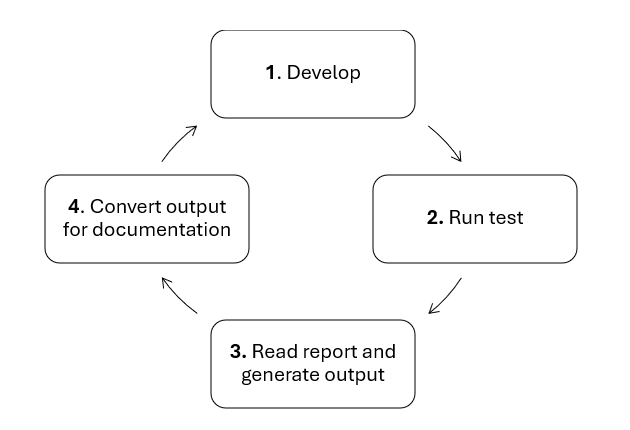
\includegraphics[width=0.6\textwidth]{../illustrations/process.png}
\end{figure}

\begin{enumerate}
    \item The first step of this cycle is, of course, development. This is the only way to move forward regarding performance. Pushing or merging new test reports should trigger a new process.
    \item Use of ReFrame for launching specified test. The results will be reported in a \textit{.json} file. If a code doesn't pass all the tests, a warning will be emitted to inform the development team of a performance decline regarding the new code.
    \item The relevant run report data will be extracted with a Python script. Then, the Python library \textit{Jinja2}\cite*{Jinja2}  generates an \textit{.adoc} file containing plotting methods.
    \item The last step is to convert the created \textit{.adoc} file into \textit{.html} for generating the website. As mentioned before, this task is performed by Antora together with AsciiDoctor.
\end{enumerate}

It's apparent that this task involves significant repetition. Therefore, we want our process to work on the most autonomous way possible.
For this point, we use the previously mentioned tools in a specific order. Each script has its role to play at a particular moment in our process timeline.
Let's see when they occur, and how they all interact together.

\begin{figure}[H]
    \centering
    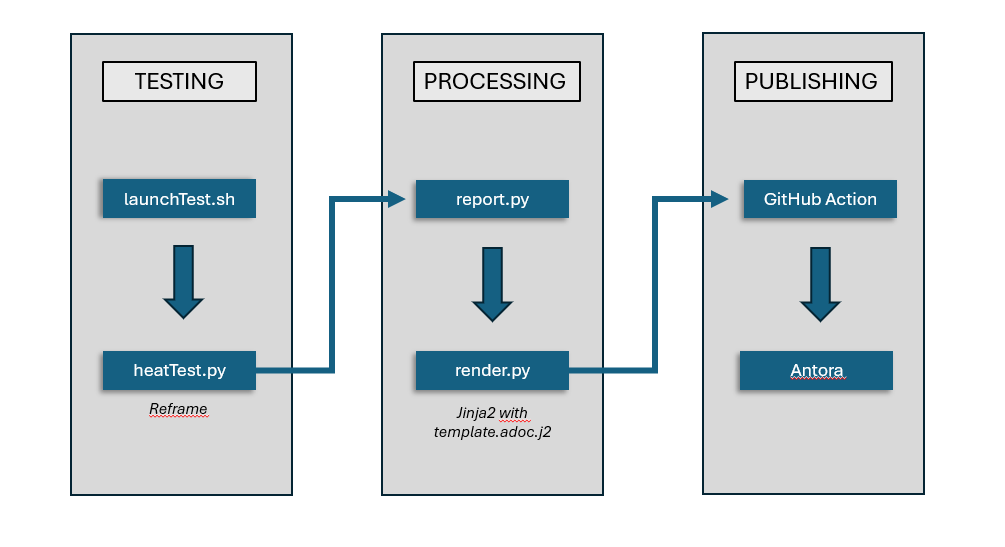
\includegraphics[width=\textwidth]{../illustrations/processWithFiles.png}
    \caption{Workflow interaction}
\end{figure}

Here follows the shell script which controls the launch of the process. In fact, it prepares the environment in which ReFrame will be launched by setting up its variables.
In addition, it makes path-issues easier to handle.\\

\begin{lstlisting}[language=bash,caption={Script for process launching}]
rm -rf ~/feelppdb
rm -rf ./build/reframe/output/ ./build/reframe/stage/ ./build/reframe/perflogs

# Variable TO BE SET to the actual HPC
hostname=gaya

current_date=$(date +%Y%m%d)
mkdir -p $(pwd)/docs/modules/${hostname}/pages/reports

export BENCH_CASES_CFG=$(pwd)/src/benchmarking/cases/

# Reframe environment variables
export RFM_CONFIG_FILES=$(pwd)/src/benchmarking/reframe/cluster-config/${hostname}.py
export RFM_REPORT_FILE=$(pwd)/docs/modules/${hostname}/pages/reports/ \
                                            ${hostname}-${current_date}-{sessionid}.json
export RFM_PREFIX=$(pwd)/build/reframe/

reframe -c ./src/feelpp/benchmarking/reframe/regression-tests/heatTest.py \
        -r --system=${hostname} --exec-policy=serial
\end{lstlisting}

\begin{tabular}{|l|m{14cm}|}
\hline
\textbf{Line} & \textbf{Description} \\
\hline
2-3  & Removing older reports and logs for avoiding unwanted interactions \\
\hline
6    & Set up the current machine \\
\hline
8    & Get date for reports naming schema \\
\hline
9    & Create reports folder if it doesn't already exist \\
\hline
11   & Export testcases path \\
\hline
14-18   & Export ReFrame environment variables: cluster configuration, report-file with naming schema, output and stage directory\\
\hline
20   & Launch Reframe recursevly \textbf{-r} on test defined in the \textit{checkpath} \textbf{-c} with the specified \textit{system}.\\
     & \textbf{--exec-policy=serial} has been set for avoiding some bugs during file access. \\
\hline
\end{tabular}

\vspace{1cm}

\section{Benchmarking with ReFrame}

\subsection{Context}
As previously mentioned, ReFrame has the capacity to focus only on the algorithm's performance, operates with Python classes that are customizable through parameterization.
Within these classes, one can easily describe and define the environment, but also parametrize the test.
General attributes like test description or file-paths can be immediately set up.

ReFrame works with an exact pipeline through different test stages, therefore the necessity to use the decorators provided by the framework.
With these decorators, Reframe schedules the execution of each method.
For each 6 different stages, going from "Initialization Phase" to "Cleanup Phase", it is possible to specify to Reframe when to execute the method.
For instance, if you want to set up the test environment, the method should probably be decorated by \texttt{@run\_before('run')}.

The site on which the test will run has to be described in a Python dictionary (or in a .json file).
It's divided into two main categories: systems and environments. \\
In the first one you can describe the specific system on which the test will be launched.
In the environment category, you can define various execution environments, for example, by specifying different compilers.

\newpage
Here is the site configuration script for Gaya, a machine located at the University of Strasbourg:

\begin{lstlisting}[language=python,caption={Gaya configuration}]
site_configuration = {
        'systems': [
            {
                'name': 'gaya',
                'descr': 'Gaya',
                'hostnames': ['gaya'],
                'modules_system': 'nomod',
                'partitions': [
                    {
                        'name': 'public',
                        'scheduler': 'squeue',
                        'launcher': 'mpiexec',
                        'max_jobs': 8,
                        'access': ['--partition=public'],
                        'environs': ['env_gaya'],
                        'processor': {
                            'num_cpus_per_socket': 64,
                            'num_sockets': 2
                        },
                        'devices': [
                            {
                                'name': 'cpu_node',
                                'num_devices': 6
                            }
                        ]
                    }
                ]
            }
        ],
        'environments': [
            {
                'name': 'env_gaya',
                'cc': 'clang',
                'cxx': 'clang++',
                'target_systems': ['gaya:public']
            }
        ]
    }
\end{lstlisting}

\begin{itemize}[left=1cm]
    \item \textit{For more specific clusters of tests, it is perfectly possible to split the system by partition, and to have multiple environments.}
    \item \textit{Specific node-lists can also be set for the test.}
\end{itemize}

The tests can be parametrized by the system's topology, which includes the number of CPUs, tasks per node, \ldots, or even by various test files. \\
For the scalability tests, the most important characteristics are the number of nodes, the number of task per core and the number of task. \\

Our tests will run with the \texttt{-bind-to core} option from \textit{mpiexec} for maximum efficiency.
Therefore, we need to know the number of physical CPUs per node. This number is given by multiplying the number of sockets by the number of CPUs per socket.
For Gaya, we can see that we have 6 nodes, with 128 physical CPUs each.

Here follows the Python function that allows to launch the testcases with different combination of nodes and number of task per core.
Numerous test cases are launched with just one command, this is precisely where Reframe's strength lies. \\

\begin{scriptsize}
\begin{lstlisting}[language=python,caption={Task number parametrization}]
def parametrizeTaskNumber():
for part in rt.runtime().system.partitions:
    nbTask = 1
    nbPhysicalCpus = part.processor.num_cpus_per_socket * part.processor.num_sockets
    while nbTask < nbPhysicalCpus:
        yield nbTask
        nbTask <<= 1

    nbNodes = part.devices[0].num_devices
    for i in range(1, nbNodes+1):
        nbTask = i*nbPhysicalCpus
        yield nbTask
\end{lstlisting}
\end{scriptsize}

\textit{This script was adapted from the 2022 CSCS Webinar \cite{CSCS} about ReFrame. \\
        We use the \texttt{reframe.core.runtime} module to access the current host's topology and the yield feature to parametrize each test by calling this function.}



For verifying the sanity of a test, Reframe provides \textit{"sanity functions"}. These functions run once the test is complete and can, for example, perform checks on the output data to ensure correctness. 
This feature enhances the reliability of our testing process, helping to catch any anomalies or errors in our results. \\
In order to avoid any regression in performance, we also have the possibility to provide references for each system configuration.


\subsection{Scale performances extraction}

With the command-line option \small{\texttt{--heat.scalability-save=1}}, or more generally \\ \small{\texttt{--<tbprefix>.scalability-save=1}}, it is possible to save scale performances from the different \textit{Feelpp toolboxes}. \\
In order to extract values from files or directly from the terminal output, we use Reframe's sanity module, particularly \texttt{sanity.extractsingle()}.
This method will extract values using \textit{regex patterns}. Methods for performance measures needs the decorator \small{\texttt{@performance\_function}}.

Explanation using an example:
\begin{scriptsize}
\begin{verbatim}
valPatt  = '([0-9e\-\+\.]+)'

@performance_function('s')
def extract_constructor_scale(self, index=1):
    scalePath = os.path.join(self.feelLogPath, 'heat.scalibility.HeatConstructor.data')
    return sn.extractsingle(rf'^{self.num_tasks}[\s]+{self.valPatt}[\s]+{self.valPatt}[\s]+{self.valPatt}[\s]
                            +{self.valPatt}[\s]+{self.valPatt}[\s]+{self.valPatt}[\s]+{self.valPatt}[\s]+{self.valPatt}[\s]+',
                            scalePath, index, float)
\end{verbatim}
\end{scriptsize}

\begin{itemize}
    \item The \small{\texttt{namePatt}} pattern is enclosed by parentheses, indicating that values corresponding to the pattern will be saved
    \item \small{\texttt{namePatt}} matches numbers, but also numbers in scientific notation
    \item Only the value at the n-th index of the corresponding pattern will be extracted
    \item The \^{} character guarantees that the pattern matches an expression starting on a new line for avoiding any unintended interaction
    \item It is necessary to know the number of values you are extracting in order to build the pattern (8 values for the feelpp\_heat\_toolbox constructor's scale)
\end{itemize}


\subsection{Process extracted data}
Reframe's results are stored in a \textit{.json} file. However, before we can properly analyze this data, we need to extract and process the information contained in the report.
This task will be performed by the \small{\texttt{Report}} class. Using the \textit{json} Python library, the class will load the report file and construct the following dataframes :
\texttt{df\_perf, df\_partialPerf, df\_speedup, df\_partialSpeedup}.

\begin{itemize}
    \item The first two dataframes will be built while reading ReFrame's report as their values are immediately reported by ReFrame
    \item The second dataframe will be built by expanding a reference value to a higher number of tasks.
    The reference value is chosen as the performance from the test with the lowest number of tasks.
\end{itemize}

Some reports do not include values for partial performance variables, but only the total score of a particular execution stage.
Therefore, we had to construct two different frames to organize the data more efficiently.
This organization facilitates comparisons between each stage component performance, especially for plotting the results.


\section{Results}

\textit{The following study has been done on case3 from Thermal Bridges ENISO10122. This is as 3-dimensional case with temperature distribution and heat flows through the wall-balcony junction.}
\textit{In order to have more calculation, the mesh 'hsize' has been passed from 0.02 to 0.01, and the discretization from P1 to P2}

\begin{figure}[h]
    \centering
    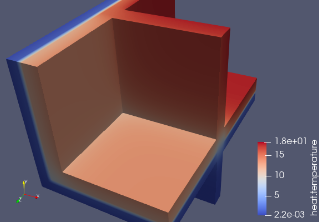
\includegraphics[width=0.3\linewidth]{../illustrations/balcony.png}
    \scriptsize{\caption{Thermal Bridges ENISO10122, Wall-Balcony\cite*{Feel++}}}
\end{figure}

\subsection{Single node test}
For single node tests, we let vary the number of task by powers of 2 up to the number of CPUs on the node. \\
As Gaya has 128 physical CPUs per node, our test were launched with 1, 2, 4, 8, 16, 32, 64, 128 tasks.

\begin{figure}[h]
    \centering
    \begin{subfigure}[b]{0.45\textwidth}
        \centering
        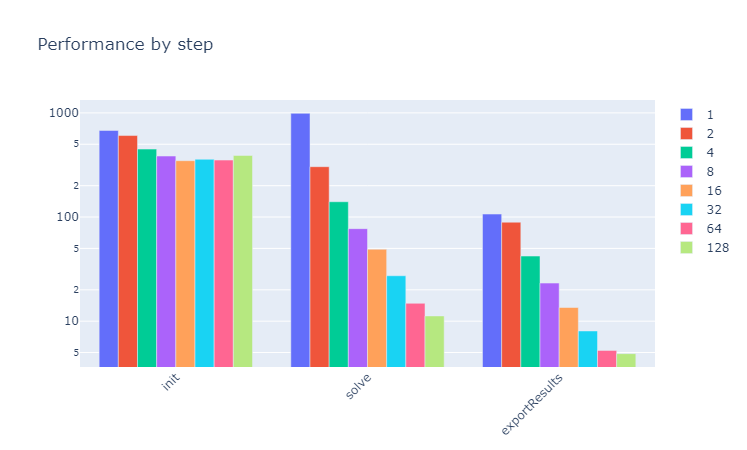
\includegraphics[width=\textwidth]{../illustrations/gaya-graphs/gayaByStep.png}
        \caption{Gaya, Performances by step}
    \end{subfigure}
    \hfill
    \begin{subfigure}[b]{0.45\textwidth}
        \centering
        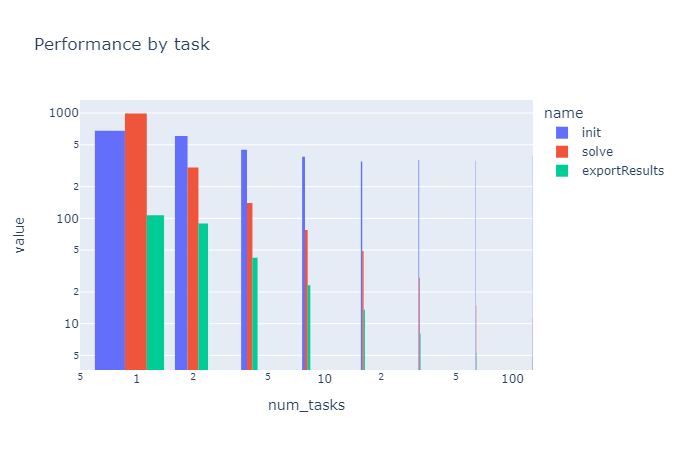
\includegraphics[width=\textwidth]{../illustrations/gaya-graphs/gayaByTask.png}
        \caption{Gaya, Performances by task}
    \end{subfigure}
\end{figure}

Both graphics represents the 3 main performance metrics, namely \textit{init, solve, exportResults} for any number of launched tasks.
We can notice that the \textit{init} stage of the process doesn't scale well, because some \textit{partial init variables} simply don't run in  parallel.
The solving and postprocessing stages scale well to higher number of tasks.

\newpage
Let's see now how the \textit{Feelpp Heat Toolbox} scales performances behaves regarding the speedup.
\begin{figure}[H]
    \centering
    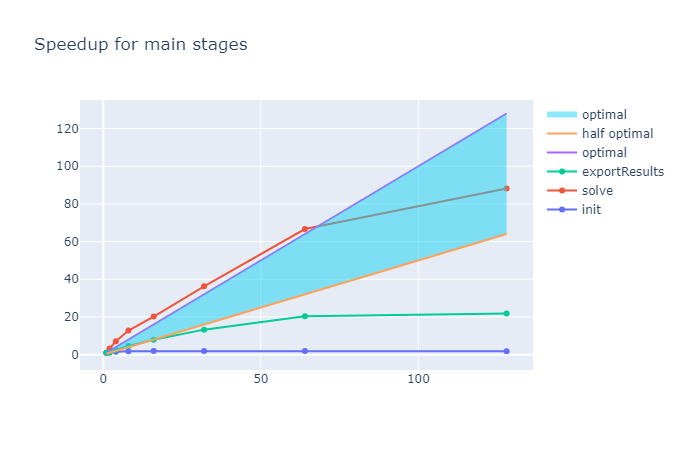
\includegraphics[width=0.7\textwidth]{../illustrations/gaya-graphs/gayaSpeedup.png}

\end{figure}

The speedup results correspond to the previous graphs.
The \textit{init} stage doesn't scale at all because of its sequential parts, while the \textit{solve} has really good performances.


\begin{figure}[H]
    \centering
    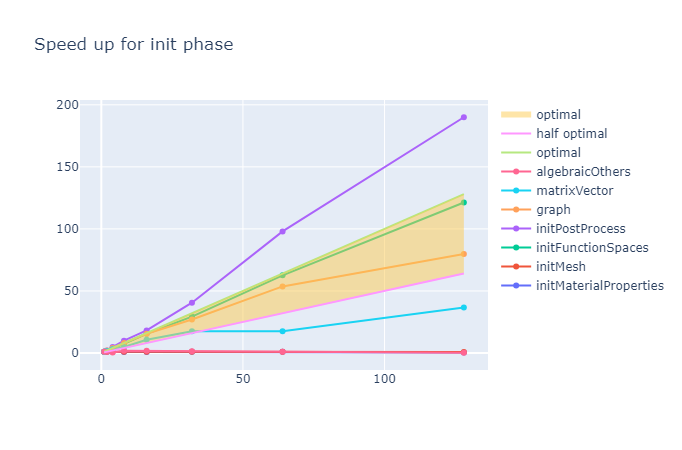
\includegraphics[width=0.7\textwidth]{../illustrations/gaya-graphs/gayaInit.png}
\end{figure}

On this illustration, we can figure out why, in the first graph, the \textit{init} phase doesn't scale well. 
The \textit{initMesh} is running in sequential, as the other curves fit in a good way to larger models. \\
This has of course a huge impact on the whole \textit{init} performance.

\begin{figure}[H]
    \centering
    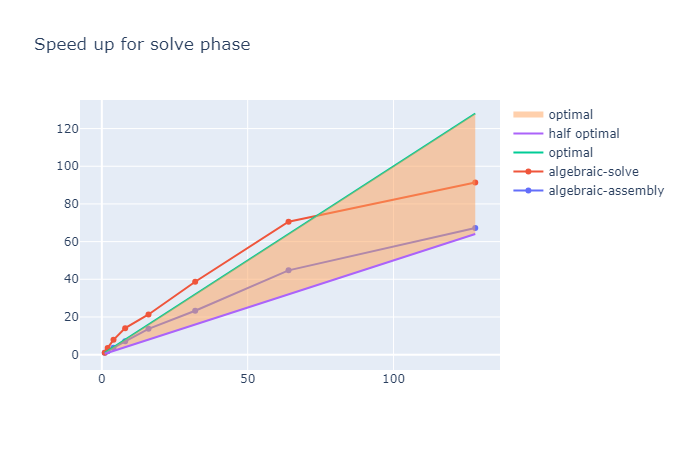
\includegraphics[width=0.7\textwidth]{../illustrations/gaya-graphs/gayaSolve.png}
\end{figure}

Even if we could think there was a problem for the values of the \textit{algebraic-solve}, because it was upon the optimal values.
The fact that it decreased with augmenting tasks number is a good sign for its aptitude to scale well.

\subsection{Multi node test}
For multi-node, we set the number of task per core to the maximum of available physical CPUs.
The total number of tasks is the product from this value with the number of nodes.

At the moment, results for multi-node testing for are not available due to an error occurring with MPI communications as soon as the number of launched task exceeds the number op CPUs per node.
Here are a few lines about this bug:

\begin{scriptsize}
\begin{verbatim}
    terminate called after throwing an instance of 'boost::wrapexcept<boost::mpi::exception>'
  what():  MPI_Test: MPI_ERR_TRUNCATE: message truncated
*** Aborted at 1716774707 (unix time) try "date -d @1716774707" if you are using GNU date ***
terminate called after throwing an instance of 'boost::wrapexcept<boost::mpi::exception>'
*** SIGABRT (@0x10fa00158edd) received by PID 1412829 (TID 0x7fc557cab000) from PID 1412829; stack trace: ***
\end{verbatim}
\end{scriptsize}

Feelpp works with the Boost.MPI library, but it seems as the communication between processes doesn't occur well.
The dev-team is already working on it.

\newpage
\section{Bibliography}
\nocite{*}
\printbibliography[heading=none]
\end{document}